% Workshop draft — §3. Independent of intro wording.
% Numbers: output/spherical_set/metrics.json and polar_texture.json
% (CVRG-Pano val∪test). Occupancy is not the spherical metric.
% Polar-texture ρ stays a failed predictor. route_plain ρ is exploratory.

\section{Latitude Weighting Is Principled and Small}
\label{sec:spherical}

The obvious geometric correction to ERP seam carving is to multiply
gradient energy by $\cos\phi$, so a pixel near the pole is not treated
as a wide equatorial step. Polar \emph{occupancy}---the fraction of
seam pixels in the top and bottom $15\%$ of rows---cannot measure that
correction: any vertical seam occupies that band at a rate fixed by the
band height (here $0.297$). The spherical signal is polar
\emph{routing share}: the fraction of cyclic $|\Delta x|$ whose starting
row is in the band. We compare plain Sobel to Sobel$\times\cos\phi$ on a
held-out outdoor set, cyclic DP both sides, and ask whether routing
rises. It does, consistently and by very little.

\paragraph{Protocol.}
CVRG-Pano official val$\cup$test ($n=120$), not cherry-picked. Same
cyclic $8$-connected DP, $24$ seams, width $\le 512$, polar band $15\%$.
Only the energy changes: unweighted Sobel versus Sobel$\times\cos\phi$
($\lambda_g=\lambda_p=1$, $\lambda_s=0$). Occupancy is the polar-pixel
fraction. Routing share uses the seam's own width so a wrap step stays
$1$\,px. Mean polar step is mean cyclic $|\Delta x|$ on polar-band rows.
The gate, locked before the run: occupancy $\max|\mathrm{diff}|<0.02$,
mean $\Delta$ routing $>0$, and a majority of images with spherical
routing $>$ plain.

\begin{table}[t]
\centering
\caption{Polar occupancy is identical by construction. Routing share is
the spherical measurement. $n=120$ CVRG val$\cup$test, $k=24$.}
\label{tab:spherical}
\begin{tabular}{lccc}
\toprule
Method & occupancy & routing share & mean polar $|\Delta x|$ \\
\midrule
Plain Sobel, cyclic & $0.297\pm 0$ & $0.301\pm 0.015$ & $0.766$ \\
Sobel $\times\cos\phi$, cyclic & $0.297\pm 0$ & $0.306\pm 0.014$ & $0.772$ \\
Paired $\Delta$ & $0.000$ & $+0.0042\pm 0.007$ & $+0.007$ \\
\bottomrule
\end{tabular}
\end{table}

\paragraph{The gate passed. The effect is small.}
Occupancy is bit-identical ($0.297$ both; $\max|\mathrm{diff}|=0$).
Routing rises from $0.301$ to $0.306$: mean $\Delta=+0.42$\,pp, $89/120$
images up, $31$ down, no ties. Mean polar step moves $+0.007$\,px.
Direction is as predicted. Magnitude is $+0.42$ percentage points on a
$\sim 30\%$ baseline; only $23/120$ images ($19\%$) move by more than
$+1$\,pp. Outdoor poles on this set are often already cheap (sky), so
$\cos\phi$ has little extra work. Both sentences belong here: the
control is real, and the size is small.

\paragraph{Polar texture does not predict the $\Delta$.}
The pre-registered content predictor was unweighted Sobel mean in the
polar $15\%$ divided by Sobel mean on the equator, measured on the same
$W\le 512$ image used to carve. Support required Spearman $\rho\ge 0.30$
and a higher mean $\Delta$ in the high-texture tercile than in the low.
The predictor has range: polar/equator Sobel runs $0.14$--$0.74$. It
still does not track $\Delta$ (Spearman $\rho=-0.01$). High-texture
tercile mean $\Delta$ is $+0.43$\,pp versus $+0.41$\,pp in the low; the
$23$ images with $\Delta>+1$\,pp have the same polar ratio as the rest
($0.359$ vs.\ $0.360$). This is a genuine null, not a no-range artifact.

Separately, every image has polar cheaper than the equator (ratio
always $<1$). The expensive-pole regime the hypothesis needed---
structured ceilings, buildings in the caps---is empty on outdoor CVRG.
Failing the predictor here does not license treating that empty regime
as a substitute pass.

\begin{figure}[t]
  \centering
  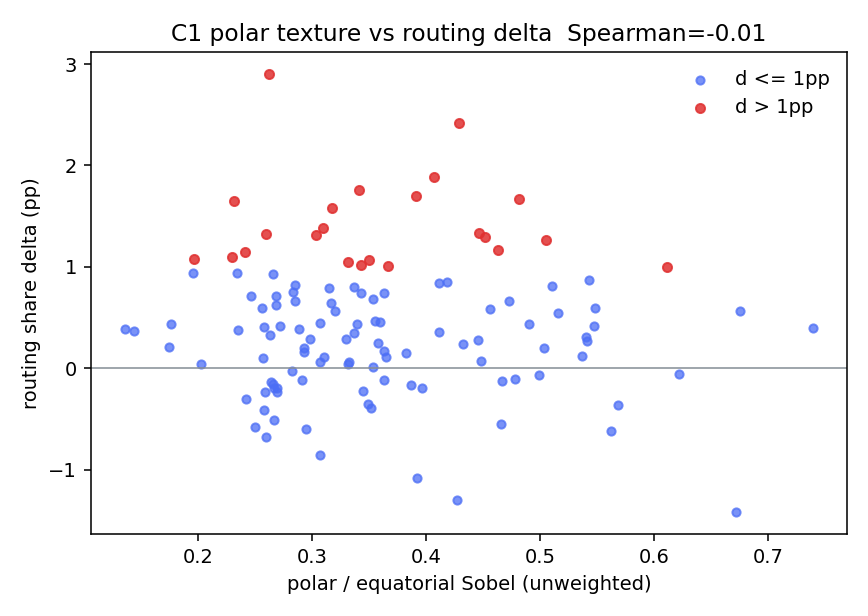
\includegraphics[width=0.82\linewidth]{figures/fig_c1_polar_scatter.png}
  \caption{Unweighted polar/equator Sobel versus routing $\Delta$
  ($n=120$). Spearman $\rho=-0.01$. Red: $\Delta>+1$\,pp. The
  $>1$\,pp tail is not the high-texture side of the predictor.}
  \label{fig:c1-scatter}
\end{figure}

\paragraph{Exploratory only.}
Routing under plain Sobel versus $\Delta$ is Spearman $\rho=-0.34$:
when the naive seam already wanders in the caps, spherical has little
left to add (low-plain tercile $+0.78$\,pp vs.\ high-plain $+0.21$\,pp).
That is partly a ceiling. It was not the pre-registered content
predictor. Report it as mechanism, not as the polar-texture result.

\paragraph{What this does and does not show.}
Latitude weighting does what the routing metric says, modestly, on $120$
outdoor ERPs, with occupancy as a sanity check rather than an outcome.
It is not a large pole-walk on real outdoor data, and it is not
``spherical helps when the pole has content''---that prediction failed
on a predictor that had range, in a set that never contained expensive
poles. The geometric term remains principled. On this corpus it is
nearly redundant.
